\documentclass{article}
\usepackage[utf8]{inputenc}
\usepackage{acl2015}
\usepackage{times}
\usepackage{url}
\usepackage{latexsym}
\usepackage{amsmath}
\usepackage{amsthm}
\usepackage{algorithm}
\usepackage[noend]{algpseudocode}
\usepackage{graphicx}

\newtheorem{theorem}{Theorem}
\newtheorem{lemma}[theorem]{Lemma}

\makeatletter
\def\BState{\State\hskip-\ALG@thistlm}
\makeatother

%\setlength\titlebox{5cm}

% You can expand the titlebox if you need extra space
% to show all the authors. Please do not make the titlebox
% smaller than 5cm (the original size); we will check this
% in the camera-ready version and ask you to change it back.

\title{CS224W Milestone\\ Time-variant Influence Spread in Social Networks}

\author{Jingning Ji \\
  Electrical Engineering \\
  Stanford University \\
  {jingning@stanford.edu} \\\And
  Yang Zhao \\
  Electrical Engineering \\
  Stanford University \\
  {yzhao12@stanford.edu} \\\And
  Yuchen Li \\
  Computer Science \\
  Stanford University \\
  {yuchenli@stanford.edu} \\}

\date{}

\begin{document}
\maketitle

\section{Introduction}
In this project, we have studied several papers related to the influence spreading through a social network. We have compared the strength and limitations of models used in each paper, and we brainstormed the problem we want to solve and the models we are using in this project. We decided to study the problem of influence spreading in social network where the strength of influence may change over time. Our goal is to propose models that well simulates the evolution process of time-variant information diffusion, and also develop algorithm on model to search initial set that maximize influence. We have came up with 2 suitable models and we used those models to simulate the influence-spreading process on twitter and facebook data set.

The rest of this paper is organized as follows. Section 2 reviewed some previous work. The testing data set described in Section 3. The detailed analysis of two models are in Section 4 and 5. Section 6 summarized the conclusion. And finally comes the difficulties and future works in Section 7 and 8.

\section{Review of the relevant prior work}

In [1] 'The spread of behavior in an online social network experiment', the author compares different hypothesis of how behavior spreads in a social network. One hypothesis is that like disease, behavior can spread with just one contact of the “infected” node. The other hypothesis is different from the previous one, which states that spreads only happen when a node is contacting many other “infected” ones. 
%\\
%\\

In [2] 'Contagion', the author focused on one specific question: when do we get contagion under deterministic best response dynamics in binary action games? Given a local interaction system describing how players interact and their payoff matrix, the author analyzed the contagion on several simple infinite network types.
%\\
%\\

Although the paper did a good job in math definition and derivation, the model is still too simple. In real world the response is not deterministic, and the network structure is not that simple as described in paper.
%\\
%\\

In [3] 'The role of social networks in information diffusion', the author did a large experiment at Facebook, to analyze information diffusion in social networks with regard of share time, multiple sharing friends, and tie strength. One contribution of the paper is that it validates Mark Granovetter's predictions about the strength of weak ties. The intuitive reason is that strong ties are redundant in spreading as close friends usually share same interests, while weak ties have more diverse information. Another interesting concept shown in the paper is homophily, which is the tendency of individuals with similar characteristics to associate with one another. Therefore we can't infer whether one's activity is resulting from homophily or influence of friends. Most models don't consider this, which leaves a large space for developing new realistic models. 

The models used in our milestone was mainly based on the models described in [4] 'Maximizing the Spread of Influence through a Social Network'

In the paper, the authors consider social network as a medium for the spread of information, ideas, and influence among its members. Diffusion models are used to simulate the dynamics of spread of information in the social network. In considering diffusion models for the spread of an idea or innovation through a social network G, represented by a directed graph, each individual node is either active (an adopter of the innovation) or inactive. This paper focuses on settings where each node’s tendency to become active increases monotonically as more of its neighbors become active. Two basic diffusion models are discussed in this paper: Linear Threshold Model and Independent Cascade Model.

In Linear Threshold Model, a node v is influenced by each neighbor w according to a weight $b_{v,w}$ such that $\sum_{\text{w, neighbour of v}}b_{v, w} \le 1$. Each node v chooses a threshold $\theta v$ uniformly at random from the interval [0, 1]; this represents the weighted fraction of v's neighbors that must become active in order for v to become active. Given a random choice of thresholds, and an initial set of active nodes $A_0$ (with all other nodes inactive), the diffusion process unfolds deterministically in discrete steps: in step t, all nodes that were active in step $t-1$ remain active, and we activate any node v for which the total weight of its active neighbors is at least $\theta v$.

The Independent Cascade Model also starts with an initial set of active nodes $A_0$, and the process unfolds in discrete steps according to the following randomized rule: when node v first becomes active in step t, it is given a single chance to activate each currently inactive neighbor w; it succeeds with a probability $p_{v,w}$ — a parameter of the system — independently of the history thus far. If v succeeds, then w will become active in step $t+1$; but whether or not v succeeds, it cannot make any further attempts to activate w in subsequent rounds.


\section{Data collection process}
\subsection{Introduction of Data Set}
The data set we are using are the social network data set from the cs224w resource website. In particular, we used ego-Facebook and ego-Twitter data sets from the social networks section. In the following section, we are providing the visualization and statistics summary of the data set we have used.

\subsection{Statistics Summary from the Data Set}
Figure 1 shows the visualization of twitter data set 1, part of the data set we have used in our simulation process. Figure 2 shows the degree distribution of it. We can see that it is absolutely preferential attachment and roughly meets power law distribution.

\begin{figure}[H]
\centering
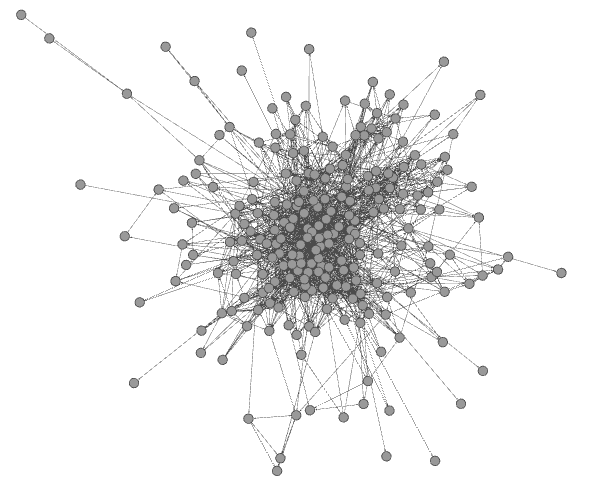
\includegraphics[width=7cm]{graph.png}
\caption{Visualization of part of Twitter data}
\end{figure}

\begin{figure}[H]
\centering
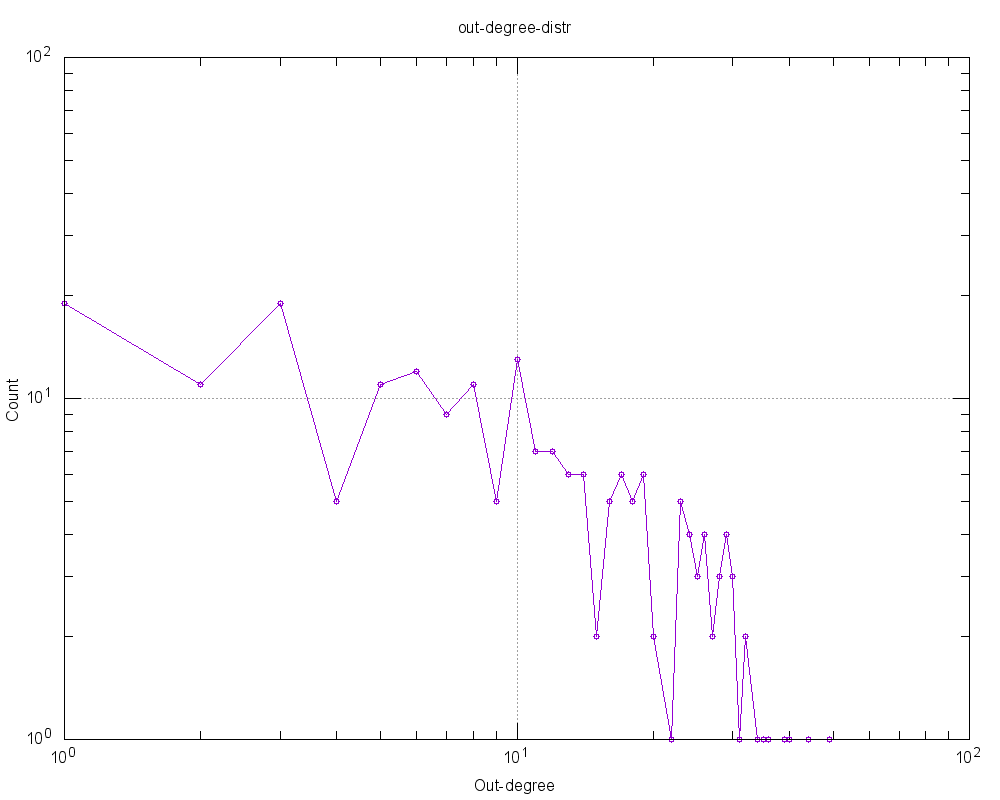
\includegraphics[width=7cm]{out-degree-distr.png}
\caption{Out Degree Distribution of part of Twitter data}
\end{figure}

\section{Simple Probabilistic Model for diffusion evolution}
\subsection{Model Description}
The model considers adoption and recovery of a person in the diffusion process. A more formal description is shown below.
\begin{enumerate}
\item Initially there are K people adopted.
\item Every time, An adopted person has probability q to recover.
\item Every time, an adopted person has probability p to infect his neighbor.
\item All people who has adopted won't adopt again.
\end{enumerate}
\subsection{Mathematical Analysis on ER network}
If a person is adopted, then the time of remaining adopting is distributed exponentially. $Pr(\tau={\tau}_0)=(1-q)^{{\tau}_0-1}q,{\tau}_0>0$ The expected time $E[\tau]=\frac{1}{q}$. The probability of a person not infecting his neighbor is $Pr(!infect)=\sum_{\tau=1}^{\infty}{(1-q)}^{\tau-1}q{(1-p)}^{\tau}=1-\frac{p}{p+q-pq}$. Therefore the probability of a person infecting his neighbor is $Pr(infect)=\frac{p}{p+q-pq}$. Therefore, this model can be regarded as a basic independent cascade model with infecting probability $\frac{p}{p+q-pq}$, without considering time. If the diffusion want to spread widely, we should have $Pr(infect)d>1$, i.e. $pd>p+q-pq$ where d is the average degree.

Then we derive the number of infected nodes by time from another perspective. Denote the number of nodes in graph by $N$, the probability of edge existing between two nodes by $s=d/N$, the expected number of adopted nodes at time t by $S_t$, the expected number of nodes having adopted at time t by $H_t$. Then at time t-1, the number of nodes that haven’t adopted is $N-H_{t-1}$. For one node that has not adopted and one node that is currently adopted, there’s probability s that an edge exists and probability p that it’s infected given the edge. Therefore, the probability of one node infected by a specific other node is $ps$. Because there are $S_t$ nodes that is adopted, the probability of an uninfected node to be infected at time t-1 is
\begin{equation}
Pr(IF_{t-1})=1-(1-ps)^{S_{t-1}}\approx 1-e^{-psS_{t-1}}
\end{equation}
Therefore, the expected number of new infected node in t is $(N-H_{t-1})(1-e^{-ps{S}_{t-1}})$. We have the following equations
\begin{equation}
H_t=H_{t-1}+(N-H_{t-1})(1-e^{-ps{S}_{t-1}})
\end{equation}
\begin{equation}
S_t=(1-q)(S_{t-1}+(N-H_{t-1})(1-e^{-psS_{t-1}}))
\end{equation}

From this equation we can also estimate a condition for diffusion to spread. When $H_{t-1}$ and $S_{t-1}$ are very small, we have 
\begin{equation}
S_t\approx(1-q)(S_{t-1}+NpsS_{t-1})=(1-q)(1+pd)S_{t-1}
\end{equation} 
To let information spread, we need $S_t>S_{t-1}$, therefore $(1-q)(1+pd)>1$, i.e. $pd>q/(1-q)$. This turns out to be too optimistic. In simulation, we need larger average degree to see the diffusion happens.

\subsection{Simulation}
First we simulated on a random generated directed ER graph, with N=236, E= 2478, p=0.2, q=0.2. For simplicity, we randomly infect one node in initialization, and set $S_0=1,H_0=1$. The simulation was run for 100 times and the average was taken. Then we simulated on a real network. The twitter network described before was chosen. The N,E,p,q were exactly the same. The theoretical curve on ER was also computed for comparison. The result is shown in Figure 3.

It can be seen that on ER graph, the theory fits pretty well with simulation result, but still overestimate the infected number. This is because we implicitly assume that the existence of edge is independent of whether the node is infected this turn, but actually they are dependent. This effect becomes larger when p is smaller than q.

Another finding is that the infected number on twitter data is less than that on ER graph. Notice the degree distribution of twitter data is more like power law distribution, and this is the main difference of two graphs. The intuition is that in a social network, there are more people having very few friends. If we initialize on them, then the diffusion will probably end quickly, and making average infected number to decrease.

\begin{figure}[H]
\centering
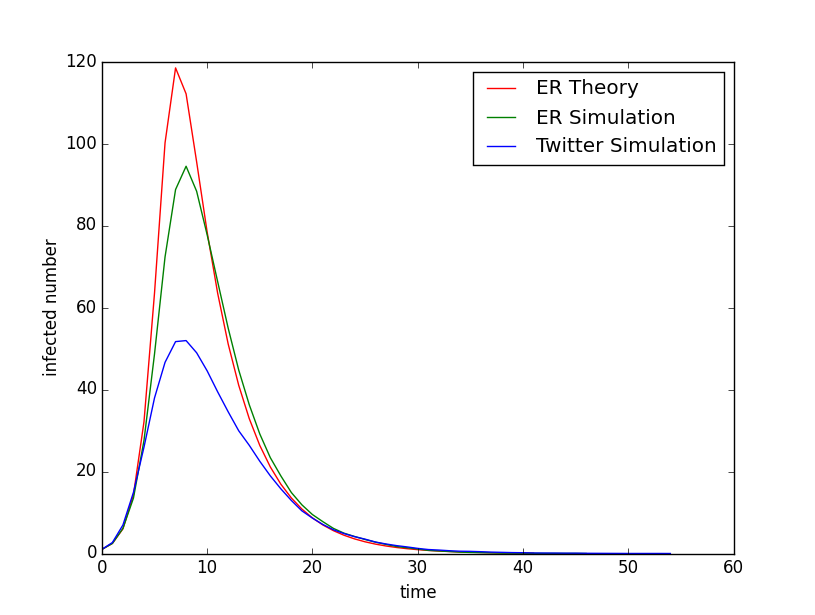
\includegraphics[width=7.5cm]{simple-plot.png}
\caption{Infected number on ER Network and Twitter Network}
\end{figure}

\subsection{Influence Maximization}
\subsubsection{Objective}
The first thing we want to talk is what should we maximize. One objective is to maximize the number of nodes that has been infected. i.e. given an initial set $I_0$, the objective function is 
\begin{equation}
f(I_0)=\lim_{\infty}H_t(I_0)
\end{equation}
where $H_t$ is the expected number of nodes which have been infected at time t, defined in Section 4.2. This is meaningful if a company want to have more people used the product. 

Another objective is to maximize the total time of all nodes being infected, i.e. the objective function is
\begin{equation}
f(I_0) = \sum_{t=0}^{t\to\infty}S_t(I_0)
\end{equation} 
where $S_t$ is the expected number of nodes being infected at time t. This will be meaningful if the product is payed by time and the company want to maximize the revenue.

The second objective is more interesting and more relevant to our model. So when we talk about influence maximization later, we refer to maximizing the total infected time. The influence maximization problem is defined as
\begin{equation}
I=\arg\max_{I_0,|I_0|\leq k}f(I_0)
\end{equation}
where k is the maximal number of nodes in initial set.

\subsubsection{Optimization Analysis}
In this simple model, since it can be regarded as independent cascade model with identical infecting time distribution, we can refer to methods used in independent cascade model.

A good choice of maximizing the influence is the greedy algorithm. In this section, we will prove that our objective function is submodular, so that the greedy algorithm can guarantee (1-1/e) performance of optimal solution.

\begin{theorem}
The objective function $f(I)$ is submodular. i.e. for all $A\subset B\subset V$ and $s\in V\backslash B$, $f(A\cup{s})-f(A)\geq f(B\cup{s})-f(B)$
\end{theorem}
\begin{proof}
For a fixed influence i, the objective function is equivalent to set paths by probability in advance and set active time by probability in advance. Since $A\subset B$, we have $H(A)\subset H(B)$, and thus $H(u)\cap H(A)\subset H(u)\cap H(B)$, $H(u)\setminus H(A)\supset H(u)\setminus H(B)$. Therefore, the gain of adding u to A is larger than adding u to B. Since the active time for each node is determined and is greater or equal than 0, the overall active time increase also have the property.

Since $f_i$ is submodular, $f$ is also submodular.
\end{proof}

The above proof shows that even we add time variable in the model and use time related objective function, the greedy algorithm will still guarantee good result.

\subsubsection{Optimization Simulation}
The greedy algorithm is simulated in this section. The greatest difficulty is that computing the objective function is hard even we know the initial set. Consider the graph as a probabilistic graphical model, it is even NP-complete problem to compute the probability of a node being infected. To address this problem, we use Monte Carlo method. The influence process is simulated for 400 times and average objective value is used in optimization. 

Because we simulated many times and take average, the optimization time will be very long. To speed up the greedy algorithm, lazy hill climbing is used by re-evaluating marginal increase only when it's necessary. 

Besides the naive (1-1/e) upper bound, we also computed the data dependent upper bound $f(I)+\sum_{i=1}^k \delta(i)$ where $\delta(i)$ is the top i marginal gain.

Other two alternative algorithms are tested in the simulation for comparison. The degree algorithm is iteratively adding the the node with biggest out degree to initial set. The random algorithm is iteratively adding a random node into initial set.

Finally we do the experiment in the small twitter network, setting $p=0.05$, $q=0.3$, $k=1,...,8$. The result is shown in Figure ???. It can be seen that greedy algorithm is the best approach. The data upper bound shows that greedy algorithm is pretty near the optimal solution. The random algorithm performs bad when $k=1$, but much better after $k>1$. The degree algorithm also performs pretty well in this small network. 

Because computing objective function is time-consuming, it's difficult to simulate in a large network. However, in linear threshold model the objective is deterministic and easy to compute, which is more friendly for influence maximization. We will discuss it in Section ???.

\begin{figure}[H]
\centering
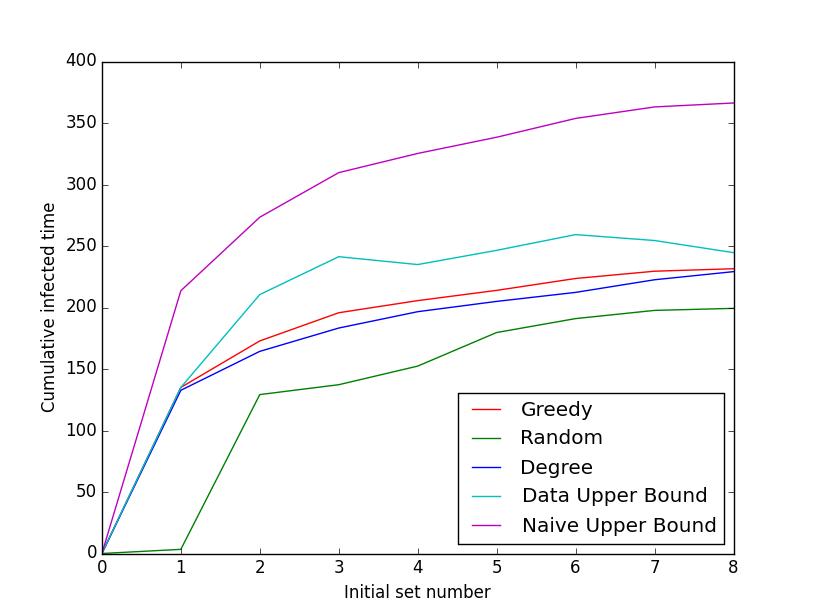
\includegraphics[width=7.5cm]{influence_max.png}
\caption{Total Infected Time by Initial Set Number}
\end{figure}

\section{Extension of Probabilistic Model}
\subsection{Variant Recover Rate}
By experience, the more a person's friends are using a product, the more likely he's going to continue using it. Therefore, we can set the recover rate q of a node to decrease by the number of its adopted friends.

\subsection{Model Extensions}
The following properties are added on top of the previous model: 
\begin{enumerate}
\item As time iteration increases, p, the probability of any node being infected by its neighbour decreases. 
\item Also the probability q such that n become inactive forever becomes larger as time iteration increases.
\end{enumerate}

This model can better describe the situation that the influence becomes weaker as time goes forward. Also it describes that people may lose interest on the subject after certain time period, therefore more likely to stop spreading. 

A simulation of this extended model over the facebook dataset is provided below:

\begin{figure}[H]
\centering
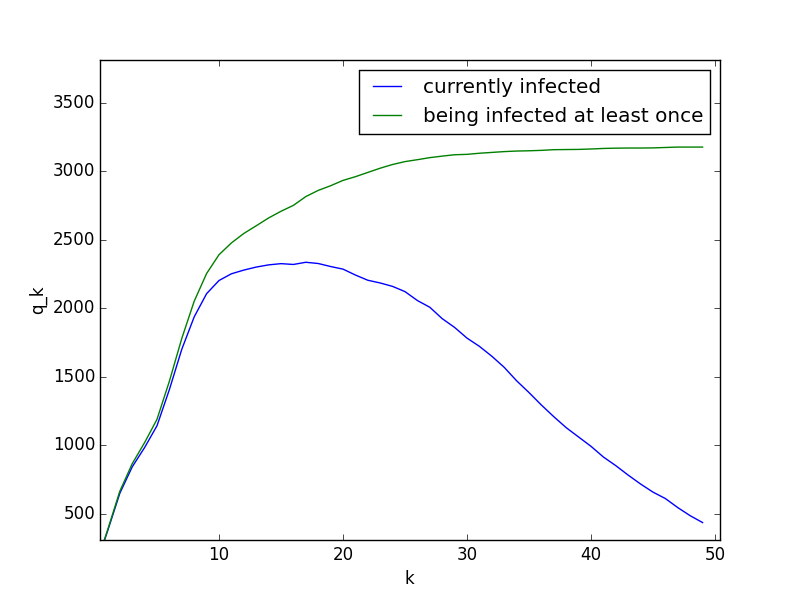
\includegraphics[width=7.5cm]{plotfb.png}
\caption{Infected number on Facebook network with extended model}
\end{figure}

\section{Time-variant Linear Threshold Model}

\subsection{Model \& Metric}
To simulate the evolution of active nodes in social network, we propose a time-variant linear threshold model based on the linear threshold model, which is described as follows:

\begin{enumerate}
\item The model is based on a graph where an edge from $i$ to $j$ indicates $i$ has influence on $j$. The influence value $I_{ij}$ is proportional to the number of common friends (undirected graph like Facebook) or followers (directed graph like Twitter) of $i$ and $j$. It's normalized so that the influence a node receives from other nodes sums up to 1, i.e. $\sum_{i \in j\text{'s neighbors}} I_{ij} = 1$.

\item Each node $i$ has an activeness sequence, which is a non-increasing sequence of real numbers in the range $(0, 1]$, i.e. $\{A_{ik}\}, k \in \{1, 2, ..., l_i\}$ where $1 \geq A_{i1} \geq A_{i2} \geq \cdots \geq A_{il_i} > 0$. Once node $i$ is activated, the starting activeness of the node is $A_{i1}$. Then, after a time step, its activeness becomes $A_{i2}$ and so forth until its activeness reaches the end of the sequence ($A_{il_i}$) and then deactivated. For inactive nodes, their activeness are 0. $l_i$ is the length of the activeness sequence of node $i$ and let's call this active time.

\item Each node $j$ has a threshold $T_j$ in the range [0, 1].  At each time step, for any node $j$, it receives activeness from its neighbors. The activeness it receives is $\sum_{i \in j\text{'s neighbors}} A_iI_{ij}$ where $A_i$ is the activeness of node $i$ in the last time step. If $\sum_{i \in j\text{'s neighbors}} A_iI_{ij} > T_j$ and node $j$ was inactive, then node $j$ is activated.

\item Each node $i$ has an upper bound of times to be activated ($U_i$) and let's call this activation upper bound. This allows a node to be activated for more than once. In default, the activation upper bound is 1, i.e. any node can be activated at most once.
\end{enumerate}

Based on the above description, by setting $\forall i, l_i = \infty, 1 = A_{i1} = A_{i2} = \cdots, U_i = 1$, this model is exactly the same as the original linear threshold model. Hence, this is a general version of linear threshold model and we can gain some insights by comparing with the original model.

In this model, we focus on the evolution of active nodes in the network instead of the total number of nodes that have been activated. To be specific, the metric for this model is the integral of number of active nodes of all time. This is more suitable for the case where reward is proportional to the length of time. For example, many online games charge players based on the playing time and thus the integral of active players is more indicative than the total number of players that have played this game for revenue estimation.

\subsection{Tests}

To test our model, we use the ego-Facebook network data, which is an undirected graph (refer to section 3 for basic statistics and visualization of this network). For simplicity, the initial set consists of users with highest degrees (let's call them influencers). The default settings are $\forall i, T_i = 0.1, l_i = 10, 1 = A_{i1} = \cdots = A_{i10}, U_i = 1$. Following are some simulation results by tweaking one of the above parameters:

\begin{figure}[!htbp]
\centering
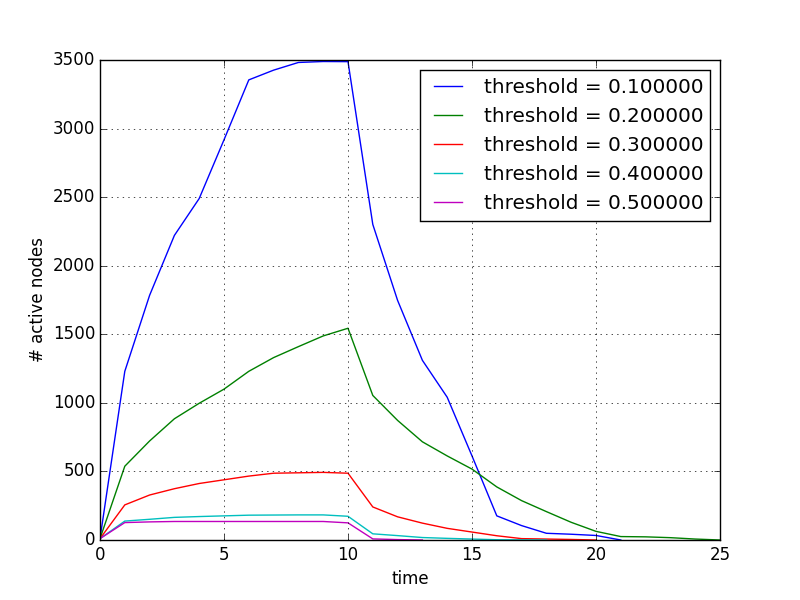
\includegraphics[width=7.5cm]{yzplot1.png}
\caption{Plot for different thresholds}
\label{threshold}
\end{figure}

In Figure \ref{threshold}, we plot the number of active nodes using different thresholds (all nodes with the same threshold). In general, when threshold increases, the number of active nodes reduces, which is reasonable because nodes are more difficult to be activated.

\begin{figure}[!htbp]
\centering
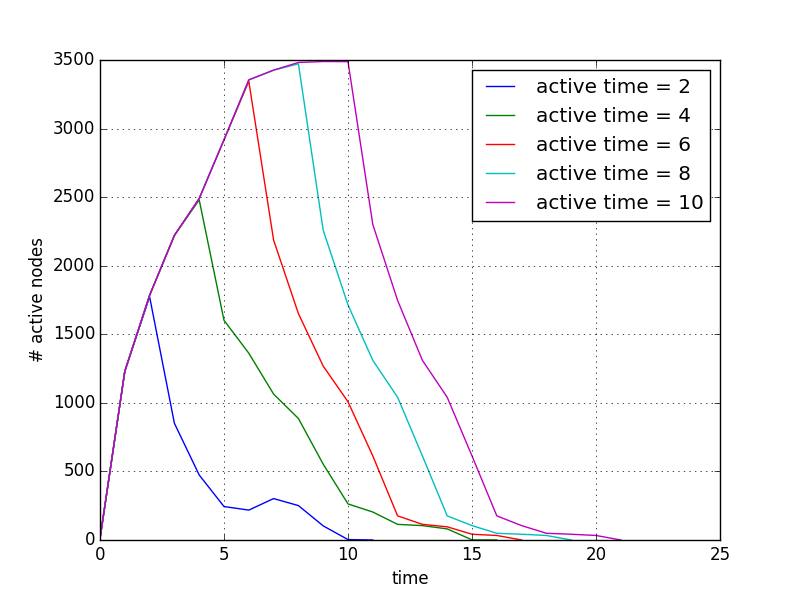
\includegraphics[width=7.5cm]{yzplot2.png}
\caption{Plot for different active times}
\label{activelength}
\end{figure}

In Figure \ref{activelength}, we plot the number of active nodes using different active times (activeness values are all 1). When active time increases, it takes longer before all nodes become inactive and the peak shifts right.

\begin{figure}[!htbp]
\centering
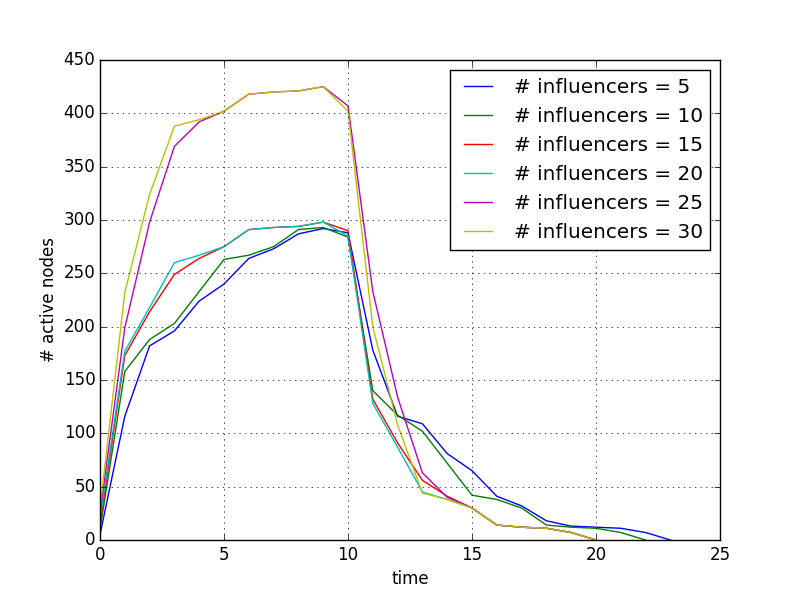
\includegraphics[width=7.5cm]{yzplot3.png}
\caption{Plot for different sizes of initial set}
\label{size}
\end{figure}

\begin{figure}[!htbp]
\centering
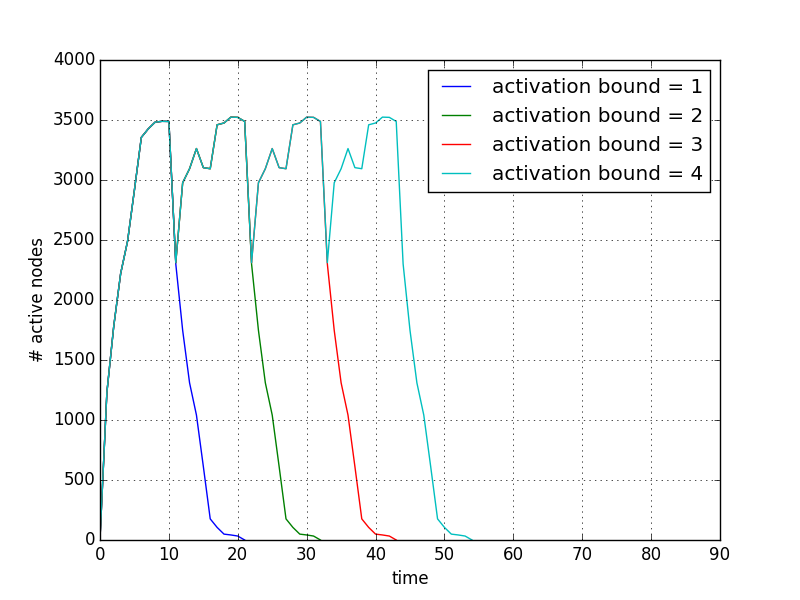
\includegraphics[width=7.5cm]{yzplot4.png}
\caption{Plot for different activation upper bounds}
\label{trigger}
\end{figure}

In Figure \ref{size}, we plot the number of active nodes using different sizes of initial set, i.e. the number of influencers. In general, when the initial set increases, the number of active nodes increases.

In Figure \ref{trigger}, we plot the number of active nodes using different trigger upper bounds. We can find the periodical change in number of active nodes in cases where the activation upper bound is larger than 1 and the period is 10, which is exactly the length of our default activeness sequence.

\subsection{Analysis \& Algorithms}

In this new model, our goal is to maximize the integral of number of active nodes over different initial sets with a given size. In the original linear threshold model, the metric is the total number of nodes that have been activated, which is proved to be a submodular function of the initial set [4]. Thus, greedy algorithm guarantees $(1 - 1/e)$ performance of the optimal solution [4].

However, the integral of number of active nodes is not submodular in the initial sets and hence greedy algorithm is not guaranteed to perform well. What's more, the scale of our data doesn't allow us to apply greedy algorithm (3963 nodes and 176312 edges) even for the singleton initial set (initial set containing only one node) because we need to enumerate all nodes, which means 3963 simulations where each one takes a few seconds.

We need to come up with other efficient algorithms to do this. Unfortunately, mathematical analysis for this problem is limited and therefore, we propose some heuristics and compare their performances in the simulation section.

The first one is the top degree heuristic, i.e. choosing nodes with highest degrees as the initial set, which we already mentioned in the previous section. This heuristic is too raw and it doesn't take the influences between nodes into consideration. For node $i$, define sum influence as $I_i = \sum_{j \in i\text{'s neighbors}} I_{ij}$, which is the sum of influences of $i$ on its neighbors. Intuitively, when $I_i$ is higher, node $i$ is more important in information spread. Based on this, we propose the top sum influence heuristic, which chooses nodes with highest sum influences as the initial set. We find that the top 10 nodes based on sum influence is exactly the 10 egos in the ego-Facebook network data, which shows that top influence heuristic is able to find the true influencers. However, top sum influence heuristic doesn't take time-related parameters into consideration. For any node $i$, during the period when $i$ is active, the total influence that $i$ spreads to its neighbors is $I_i \cdot \sum_{k=1}^{l_i} A_{ik}$ and let's call this cumulative influence. The top cumulative influence heuristic is choosing top nodes based on cumulative influence as the initial set.

\subsection{Simulation Results}

Based on the three heuristics proposed in the previous section, we run the simulation and compare their performances. For any node $i$, we set activation upper bound $U_i = 1$ and active time $l_i$ to a random integer in the range $[5, 15]$ where activeness values are all ones. For each of following simulation results, we average over 100 different models to reduce the effect of randomness (the only difference is the active time for nodes).

\begin{figure}[!htbp]
\centering
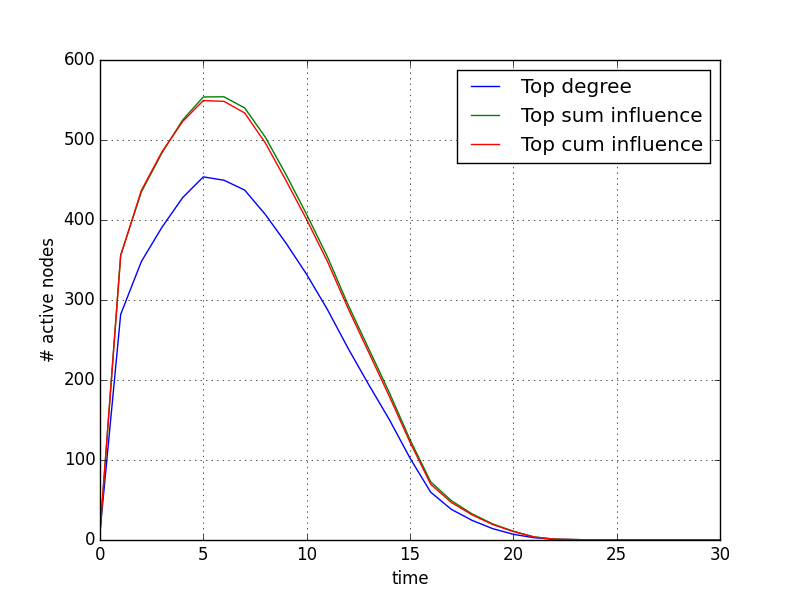
\includegraphics[width=7.5cm]{yzplot5.png}
\caption{An example comparison of three heuristics}
\label{example}
\end{figure}

In Figure \ref{example}, we show an example simulation of three heuristics, from which we can see top sum influence heuristic and top cumulative influence heuristic outperforms the top degree heuristic. What's more, the difference between top sum influence heuristic and top cumulative influence heuristic is negligible.

\begin{figure}[!htbp]
\centering
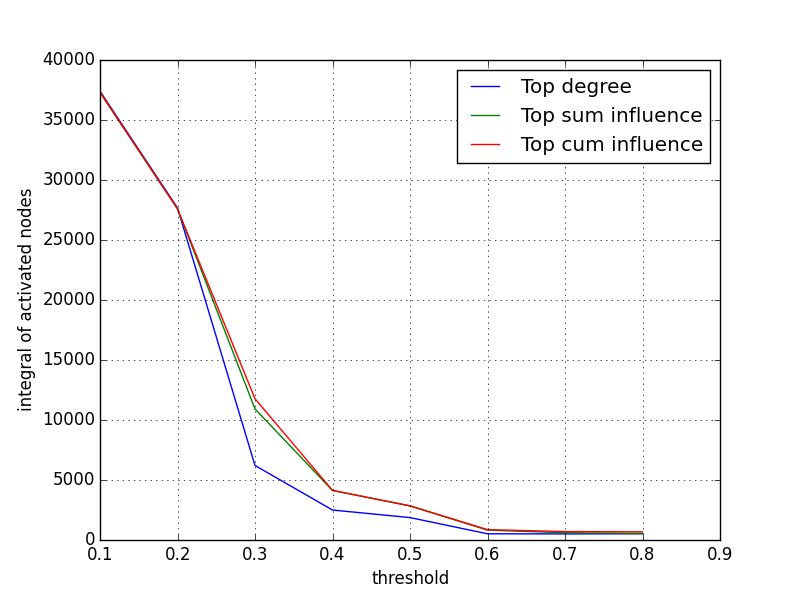
\includegraphics[width=7.5cm]{yzplot6.png}
\caption{Performance plot using different thresholds with init set size 50}
\label{pthreshold}
\end{figure}

In Figure \ref{pthreshold}, we fix the initial set size to 50 and compare the performances using different thresholds for all nodes. As expected, when the threshold increases, the integral of activated nodes reduces. The gap between top degree heuristic and the other two algorithms is the largest when threshold is 0.3.

\begin{figure}[!htbp]
\centering
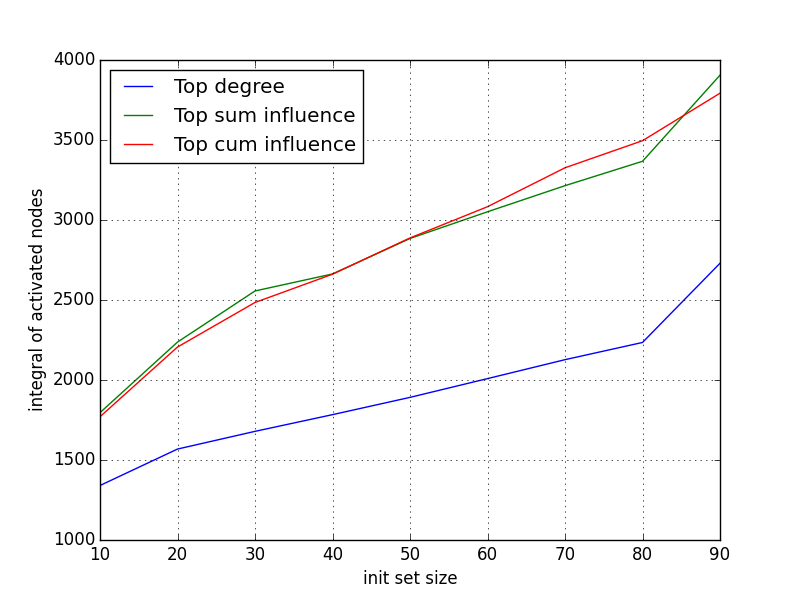
\includegraphics[width=7.5cm]{yzplot7.png}
\caption{Performance plot using different initial set sizes with threshold 0.5}
\label{psize}
\end{figure}

In Figure \ref{psize}, we fix the threshold to 0.5 and compare the performances using different initial set sizes. We can see there's a gap between top degree heuristic and the other two algorithms while the difference between the other two algorithms is still very small.

\subsection{Conclusion}

From the above simulation results, we can conclude that among the three heuristics, the top degree heuristic is the worst, which only involves degree information. The performance of the other two algorithms are very close and they outperform the top degree heuristic. To make use of the time-related parameters, we can further generalize the top cumulative influence heuristic to an algorithm that chooses top nodes based on $f(I_i, \sum_{k=1}^{l_i} A_{ik})$ where $f(\cdot)$ could be any function. We can consider $I_i$ and $\sum_{k=1}^{l_i} A_{ik}$ as features and treat this as a machine learning problem and we should achieve an algorithm that outperforms the top sum influence heuristic because this algorithm is also a special case of the above general algorithm. In the future, we need more mathematical analysis for this problem and achieve better algorithms other than heuristics.

\section{Summary}
We have constructed different models for predicting time-variant influence spread: the simple probablistic model and the time-variant linear threshold model. From the mathematical and simulation analysis, we have seen that both models are valid assumptions about how influence can spread over time in a real world situation. 

\section{Difficulties}
The main difficulties we met are as follows:
\begin{enumerate}
\item It is difficult to get a real world statistics of infecting number by time on a known graph. Therefore, it's hard to measure if a model behaves like real world.
\item The model is to too complicated to allow theoretical analysis, and also make it hard to develop influence maximization algorithms.
\item Doing simulation on a huge data set is very slow, and even inapplicable on personal computer. Currently we are simulating on relatively small data sets.
\end{enumerate}

\section{Future works}
Things that are left to do after the milestone are:
\begin{enumerate}
\item We need to determine a good algorithm of finding the best initial infected set. Right now we are just using simple heuristics of choosing infected nodes with largest centrality degree.
\item We need to perform our algorithm on a larger data set and test the run-time performance of the different algorithms.
\item Also we need to compare the different models we have used and determine the best model for predicting different real-world influence spreading situations. And based on the model we use, we will predict the future spreads on one of the real data set and gain some insights of our prediction over future influence.
\end{enumerate}
%\\
%\\
%i. We need to determine a good algorithm of finding the best initial infected set. Right now we are just using simple heuristics of choosing infected nodes with largest centrality degree.
%\\
%\\
%ii. We need to perform our algorithm on a larger data set and test the run-time performance of the different algorithms. 
%\\
%\\
%iii. Also we need to compare the different models we have used and determine the best model for predicting different real-world influence spreading situations. And based on the model we use, we will predict the future spreads on one of the real data set and gain some insights of our prediction over future influence.

\section{References}
%\begin{thebibliography}{}
%
%\bibitem[\protect\citename{{Centola}}2010]{Centola:10}
%Damon Centola.
%\newblock 2010.
%\newblock {\em The spread of behavior in an online social %network experiment}, Science
%
%\end{thebibliography}
[1] Damon Centola, The spread of behavior in an online social network experiment, Science, 2010.

\noindent [2] S. Morris. Contagion. Review of Economic Studies 67, 57-78, 2000.

\noindent [3] Bakshy, Rosenn, Marlow, and Adamic, The role of social networks in information diffusion, Proc. WWW, 2012

\noindent [4] D. Kempe, J. Kleinberg, E. Tardos, Maximizing the Spread of Influence Through a Social Network, KDD'03.

\end{document}

